        \clearpage
        \begin{figure*}[ht]
            \pdfbookmark[2]{ID 06}{figure_id_06}
        	\centering
            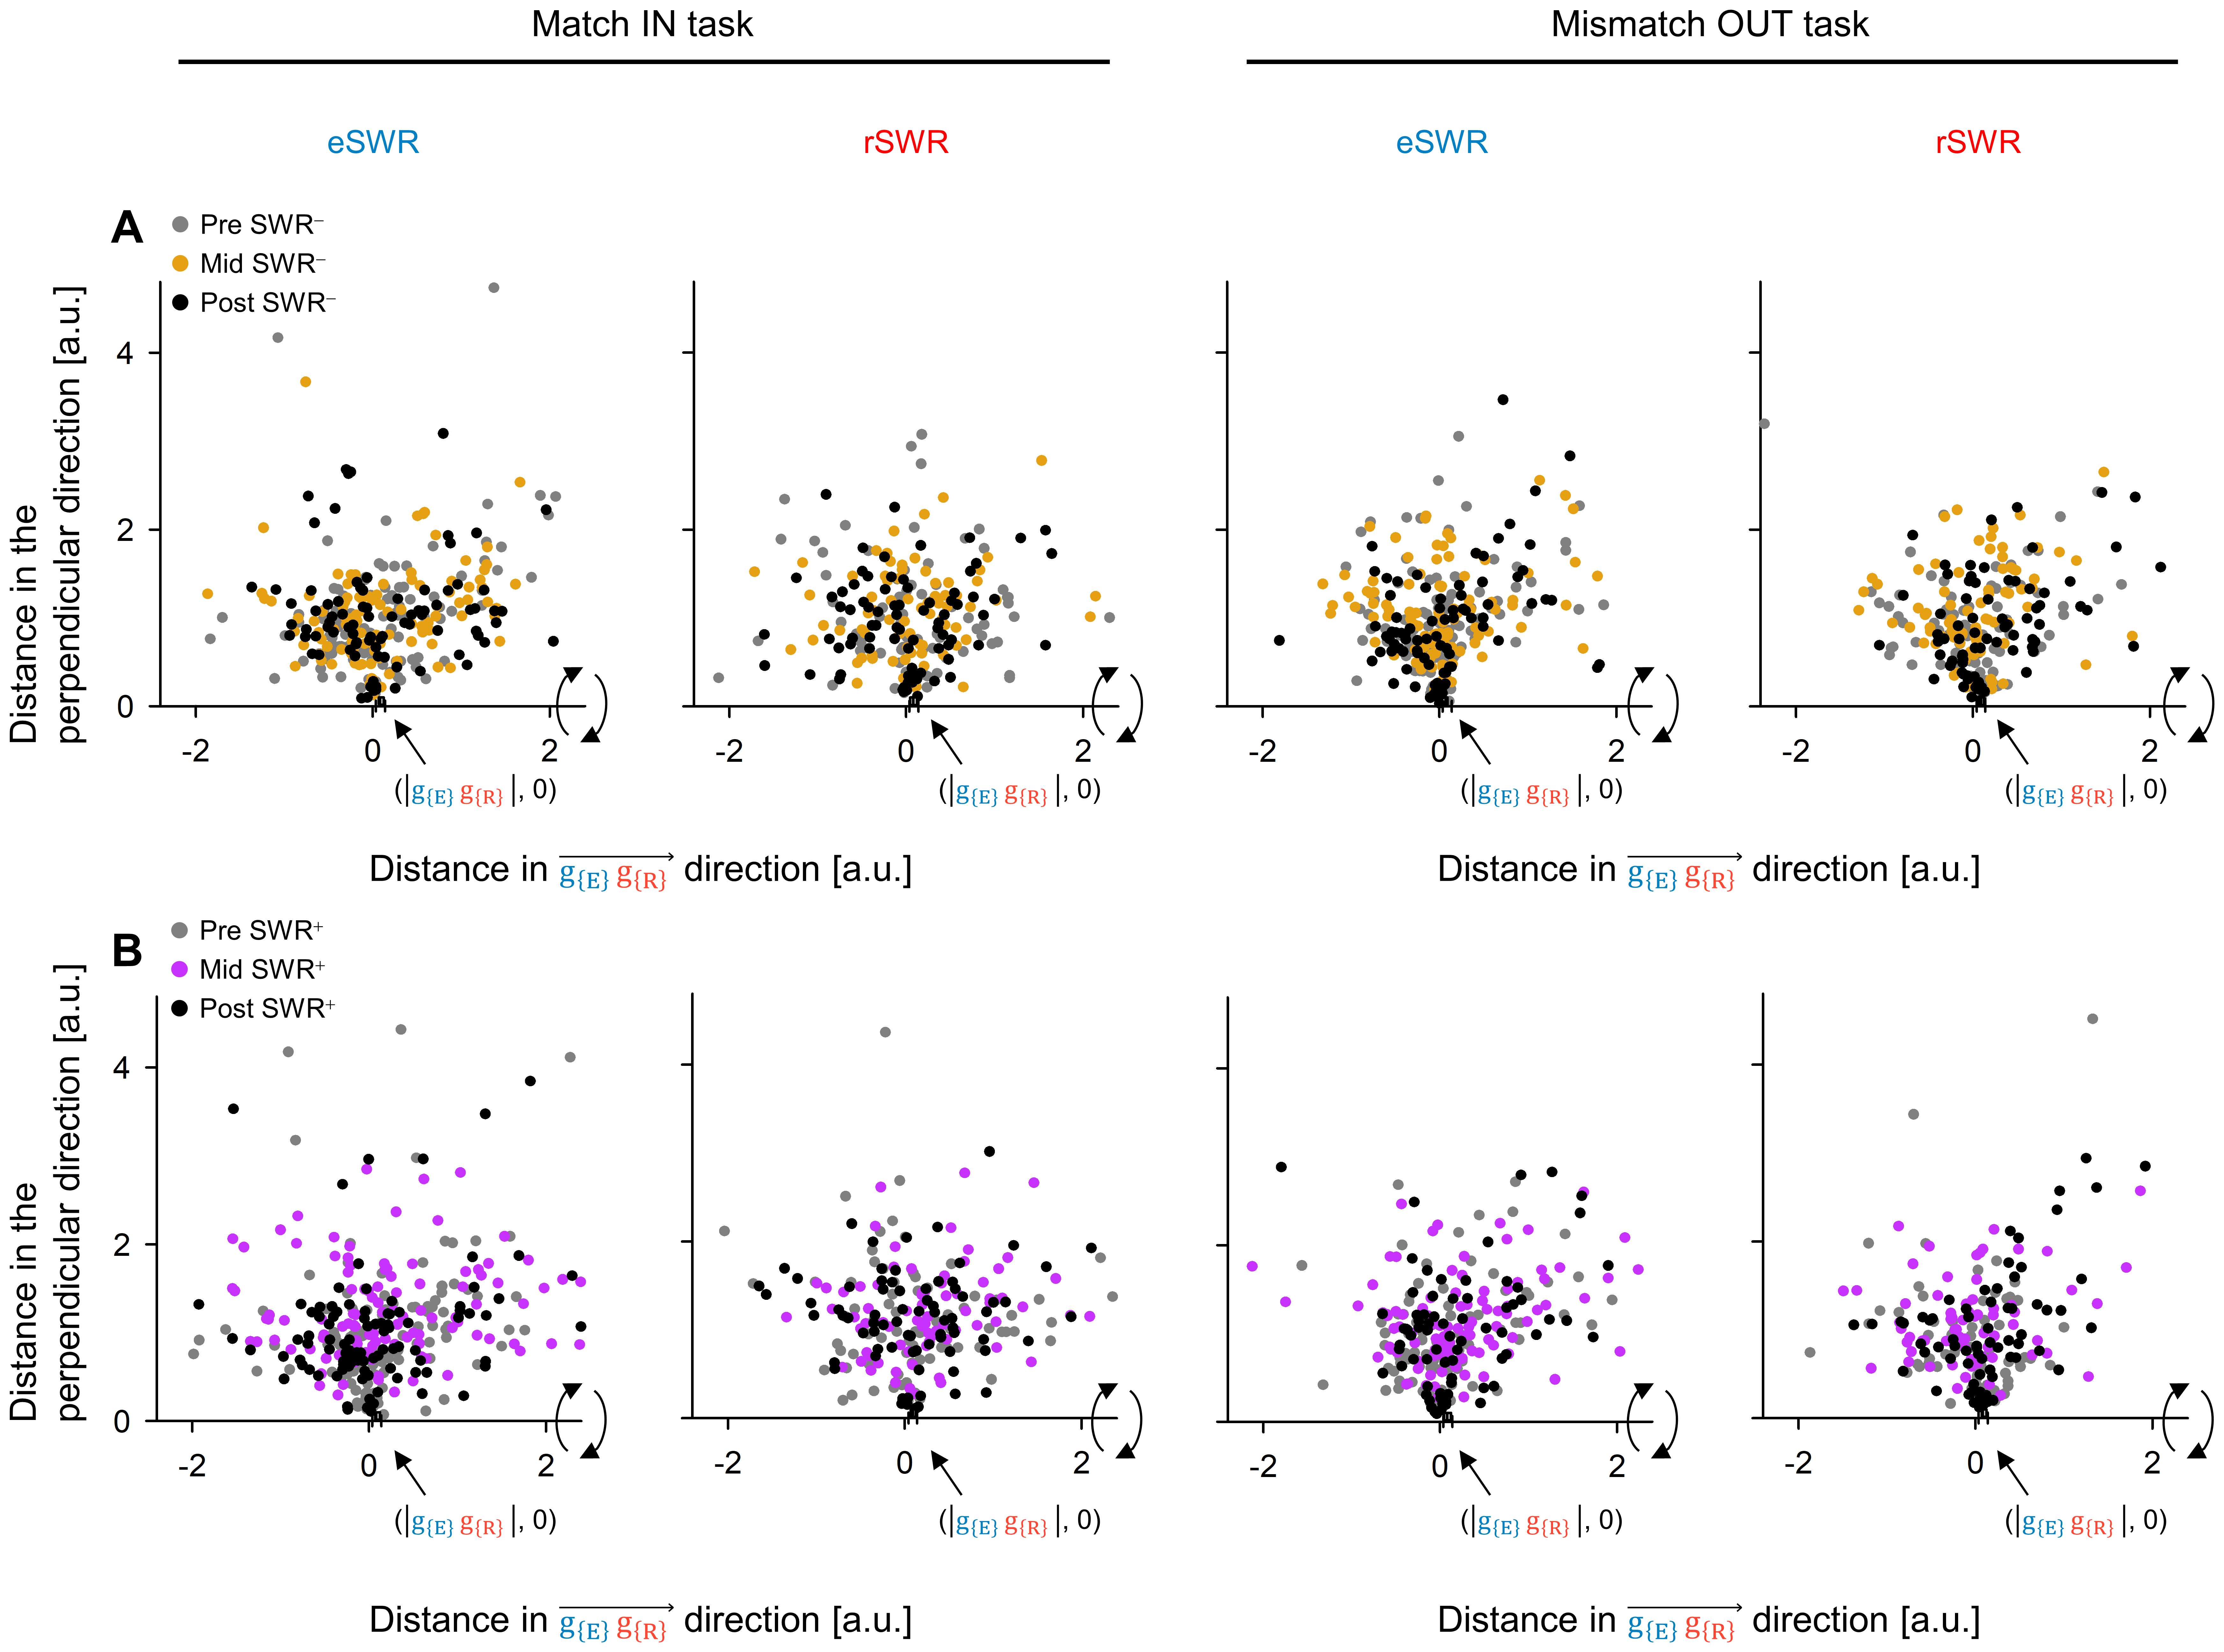
\includegraphics[width=1\textwidth]{./src/figures/.png/Figure_ID_06.png}
        	\caption{\textbf{
Visualization of Neural Trajectories during SWR in Two-Dimensional Spaces}
\smallskip
\\
The panels display hippocampal neural trajectories during SWR as projected onto two-dimensional spaces. \textbf{\textit{A.}} Indicates hippocampal neural trajectories pre-SWR$^-$ (\textit{gray}), mid-SWR$^-$ (\textit{yellow}), and post-SWR$^-$ (\textit{black}). \textbf{\textit{B.}} Represents the equivalents for SWR$^+$ as opposed to SWR$^-$. The $\lVert \mathrm{g_{E}g_{R}} \rVert$ varied among sessions. The projection was applied in the following manner: First, a linear transformation positioned $\mathrm{g_{E}}$ at the origin $O$ (0,0), and $\mathrm{g_{R}}$ at ($\lVert \mathrm{g_{E}g_{R}} \rVert$, 0). The point cloud was then rotated around the $\mathrm{g_{E}g_{R}}$ axis (equivalent to the x axis) for fitting into two-dimensional spaces. Therefore, within these two-dimensional spaces, both the distances from $O$ and the angles preserved the original makeup of the $\mathrm{g_{E}g_{R}}$ axis from the original three-dimensional spaces. Abbreviations: SWR signifies sharp-wave ripple events; eSWR denotes SWR during the encoding phase; rSWR indicates SWR during the retrieval phase; SWR$^+$, marks an SWR event; SWR$^-$ refers to control events for SWR$^+$; pre-SWR, mid-SWR, or post-SWR, reference the time intervals from $-800$ to $-250$ ms, from $-250$ to $+250$ ms, or from $+250$ to $+800$ ms from the center of SWR.
}
% width=1\textwidth
        	\label{fig:06}
        \end{figure*}
